\chapter{Численные методы и комплексы программ}\label{ch:ch3}


\section{Первая статья}\label{sec:ch3/sect1}
Пусть функционал $J(\theta)$ удовлетворяет условиям, указанным в \autoref{sec:optimality}.
Для удобства введём переобозначение $\hat{J}(u):=J(\theta(u)), \hat{J}:L^2(\Gamma_1) \to \mathbb{R}$.
Здесь $\theta(u)$ -- температурное поле задачи  \eqref{initial}--\eqref{initial-boundary} отвечающее
управлению $u \in L^2(\Gamma_1)$.
Согласно формуле \eqref{therorem_2_eq3} градиент функционала $\hat{J}(u)$~\cite{grenkin_13} имеет вид
\[
    \hat{J}'(u)= (\varphi(u) -\theta_b^4)p_2,
\]
где $\varphi(u)$ есть интенсивность излучения, $p_2$ -- соответствующая переменная сопряжённой системы.

Предлагаемый алгоритм решения выглядит следующим образом:
\begin{algorithm}[H]
    \caption{Алгоритм градиентного спуска с проекцией}
    \begin{algorithmic}[1]
        \State Выбираем значение градиентного шага $\lambda$,
        \State Выбираем количество итераций $N$,
        \State Выбираем произвольное $u_0 \in U_{ad}$,
        \For{$k \gets 0,1,2,...,N$}
            :
            \State Для полученного $u_k$ расчитываем состояние $y_k = \{\theta_k, \varphi_k\}$ из  (\ref{weak_operational}).
            \State Расчитываем значение функционала качества $J(\theta_k)$ из (\ref{quality}).
            \State Расчитываем сопряжённое состояние $p_k=\{p_{1k},p_{2k}\}$ из уравнений \eqref{therorem_2_eq1}--\eqref{therorem_2_eq2}, где $ \hat{\theta} := \theta_k, \hat{u}=u_k$.
            \State Пересчитываем управление $u_{k+1} = P_{ad}\left[ u_k - \lambda (\varphi_k - \theta_b^4)p_{2k} \right]$.
        \EndFor
    \end{algorithmic}\label{alg:algorithm}
\end{algorithm}
Оператор проекции $P_{ad} : U \to U_{ad}$ определён следующим образом
\[
    P_{ad}[v] =
    \begin{cases}
        u_1, & \text{если } v \le u_1 \\
        v, & \text{если } u_1 < v < u_2 \\
        u_2, & \text{если } v \ge u_2
    \end{cases}
\]
Приведём далее примеры расчётов для двумерного случая.
Положим $\Omega = \{(x,y), 0 \leq x,y \leq 1\}$, $l = 1$ см.
Граница $\partial\Omega$ состоит из участков:
\[
    \begin{aligned}
        \Gamma_0 & = \{x=\{0,1\}, y \in [0,1]\} \\
        \Gamma_1 & = \{x\in [0,1], y=0\} - \text{участок с неизвестными отражающими свойствами,} \\
        \Gamma_2 & = \{x \in [0,1], y=1\} - \text{участок наблюдения.}
    \end{aligned}
\]
Будем также далее считать, что $a = 0.006[\text{см}^2/\text{c}]$, $b=0.025[\text{см}/\text{с}]$, $\beta = 0.00005[\text{см}/\text{с}]$, $\kappa=1[\text{см}^{-1}]$, $\kappa_s = 0$, $A = 0$, $\gamma = 0.3$.
Указанные параметры соответствуют стеклу \cite{grenkin_13}.
Температуру на границе $\Omega$ положим равной $\theta_b = (x^2+y^2)/3$.

При указанных параметрах для первого эксперимента выберем следующее тестовое значение
функции $u$ (рис. \ref{fig:control}\subref{fig1:exp1}):
\begin{equation}
    u(x)=
    \begin{cases}
        0.01, & \text{если } x \le 0.5, \\
        0.5, & \text{если } x > 0.5,
    \end{cases}\label{eq:equation}
\end{equation}
и для второго эксперимента (рис.~\ref{fig:control}\subref{fig1:exp2}):
\begin{equation}
    \label{eq:test_function_1}
    u(x)=0.49x+0.01. \;
\end{equation}

Вычислим решение прямой задачи~\eqref{eq:initial}--\eqref{eq:initial-boundary} для этих случаев.
Полученное температурное поле на участке наблюдения $\Gamma_2$ выберем в качестве $\theta_0$.
Далее, применяя предложенный алгоритм находим квазирешение
обратной задачи~\eqref{eq:initial}--\eqref{eq:theta_gamma}.
Эффективность алгоритма, а также значение $u_0$ в первом и
втором случаях иллюстрируются рис.~\ref{fig:control}.
На рис.~\ref{fig:cost} показана динамика функционала качества по итерациям.

\textbf{Замечание.} В предложенных примерах потребовалось $2*10^6$ итераций для нахождения квазирешения $u$.
В то же время температурное поле на участке наблюдения $\Gamma_2$ становится близким
к $\theta_0$ уже на $10^2$ итерации.
Также наблюдается существенное падение скорости уменьшения функционала качества с
каждой итерацией после того, как среднее значение найденной функции контроля
становится близко к тестовой функции.
\begin{figure}[H]
    \centering
    \subfloat[Первый эксперимент]
    {
        \label{fig:exp1}
        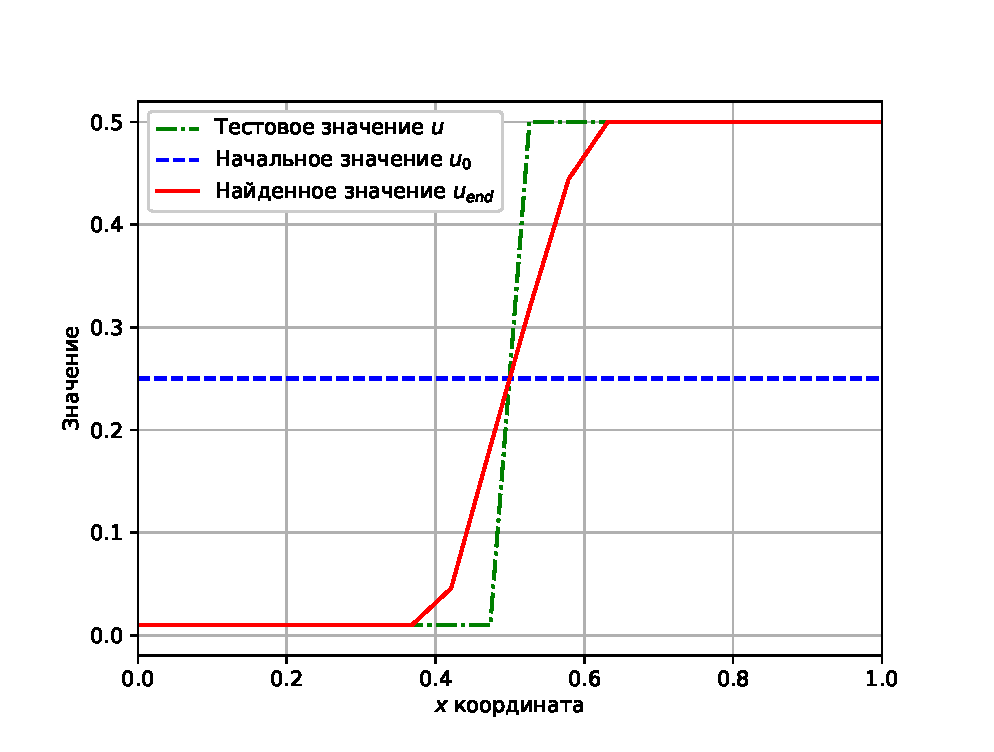
\includegraphics[width=.51\linewidth]{1.eps}
    }
    \subfloat[Второй эксперимент]
    {
        \label{fig:exp2}
        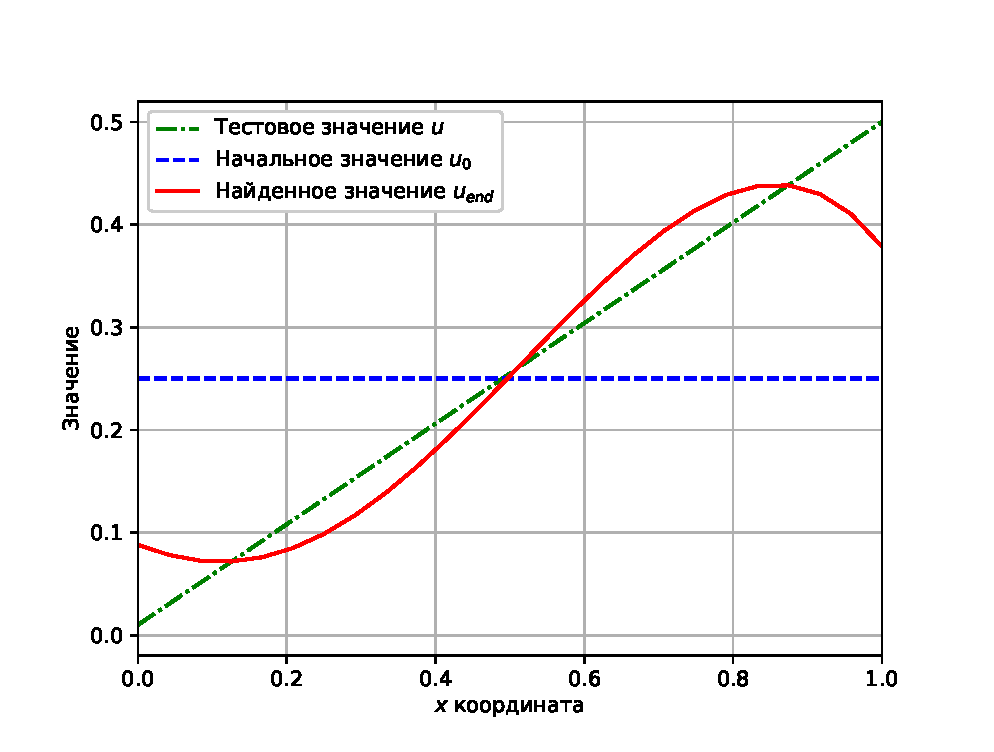
\includegraphics[width=.51\linewidth]{2.eps}
    }
    \caption{Тестовая функция $u$, начальная $u_0$, найденная функция $u_{end}.$}
    \label{fig:control}
\end{figure}

\begin{figure}[H]
    \centering
    \subfloat[Первый эксперимент]
    {
        \label{fig:exp12}
        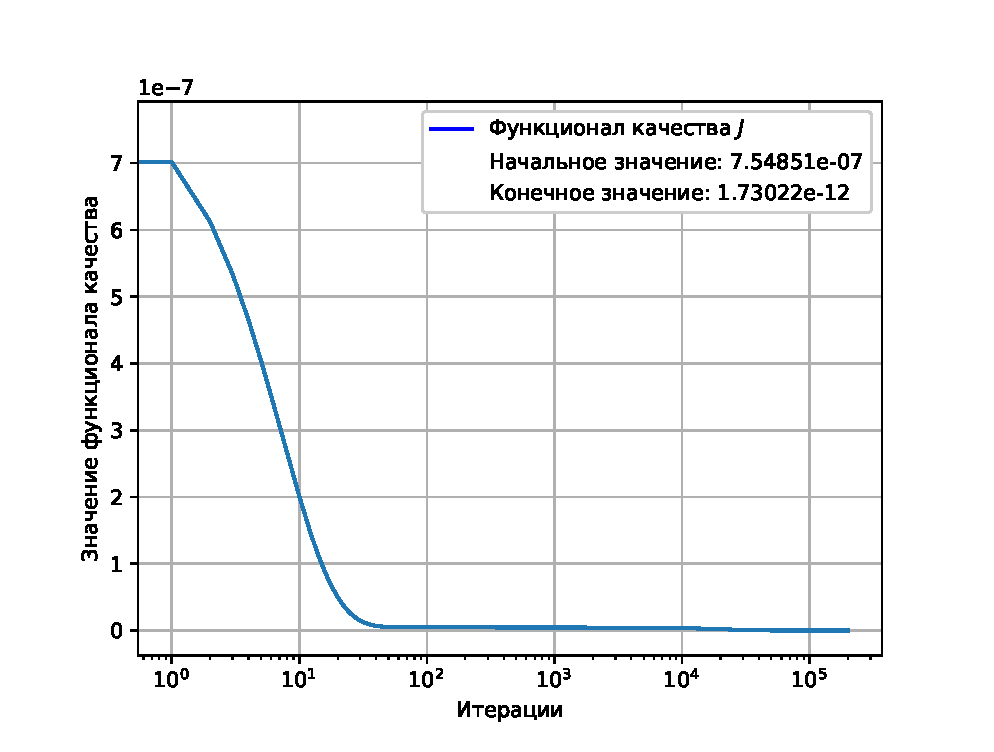
\includegraphics[width=.51\linewidth]{3.eps}
    }
    \subfloat[Второй эксперимент]
    {
        \label{fig:exp22}
        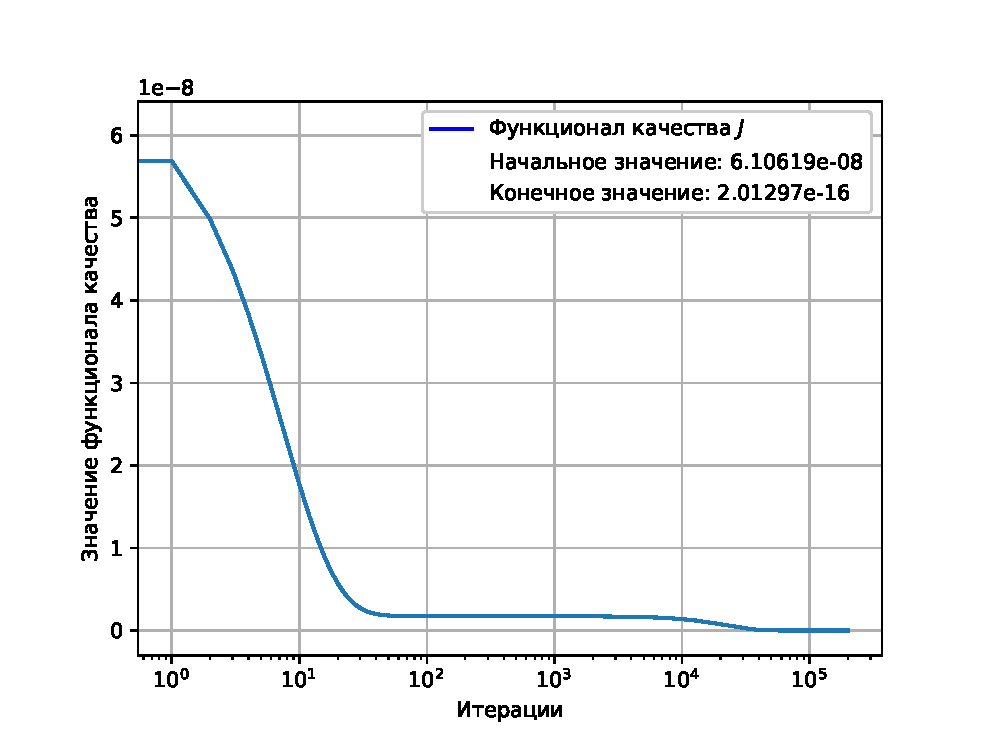
\includegraphics[width=.51\linewidth]{4.eps}
    }
    \caption{Динамика функции $\hat{J}(u)$ по итерациям.}
    \label{fig:cost}
\end{figure}

\clearpage


\section{Вторая статья}\label{sec:ch3/sec2}
\subsection{Аппроксимация задачи с условиями типа коши}\label{subsec:ch3/3_1}
Рассмотрим краевую задачу~\eqref{eq1}-\eqref{bc2} для уравнений сложного теплообмена, в которой нет краевых условий на
интенсивность излучения.
Существование $\theta,\varphi\in H^2(\Omega)$, удовлетворяющих~\eqref{eq1}-\eqref{bc2}
для достаточно гладких
$\theta_b,\, q_b$ и достаточные условия единственности решения
установлены в~\cite{CMMP20}.
Покажем, что решения задачи $(CP)$ при $\lambda\to+0$
аппроксимируют решение задачи~\eqref{eq1}-\eqref{bc2}.


\textbf{Теорема 3.}
{\it
Пусть выполняются условия} (i),(ii) {\it и существует решение задачи~\eqref{eq1}-\eqref{bc2}.}
    {\it  Если $\{\theta_\lambda,\varphi_\lambda,u_\lambda\}$ -- решение
задачи $(CP)$ для $\lambda>0$, то существует последовательность
$\lambda\to +0$
такая, что}
\[
    \theta_\lambda\rightarrow\theta_*, \;\; \varphi_\lambda\rightarrow\varphi_*
    \text{ слабо в }V,\text{ сильно в }H,
\]
    {\it где $\theta_*,\varphi_*$ -- решение задачи~\eqref{eq1}-\eqref{bc2}.}

    {\bf Доказательство.}
Пусть $\theta,\varphi\in H^2(\Omega)$ -- решение задачи~\eqref{eq1}-\eqref{bc2},
$u=\alpha(\partial_n\varphi+\varphi)\in U.$ Тогда
\[
    a A \theta + b \kappa_a ([\theta]^4 - \varphi ) = Br,\quad
    \alpha A \varphi + \kappa_a (\varphi - [\theta]^4)  = Bu,
\]
где $r:=a(\theta_b+q_b).$ Поэтому, с учетом того, что $\theta|_\Gamma=\theta_b$,
\[
    J_\lambda(\theta_\lambda, u_\lambda) = \frac{1}{2}\|\theta_\lambda -\theta_b\|^2_\Gamma
    + \frac{\lambda}{2}\|u_\lambda\|^2_\Gamma\leq J_\lambda(\theta, u)=\frac{\lambda}{2}\|u\|^2_\Gamma.
\]
Следовательно,
\[
    \|u_\lambda\|^2_\Gamma\leq C,\;\; \|\theta_\lambda -\theta_b\|^2_\Gamma\to 0,\; \lambda\to +0.
\]
Здесь и далее $C>0$ не зависит от $\lambda.$
Из ограниченности последовательности $u_\lambda$ в пространстве $U$ следуют, на основании
леммы 1, оценки
\[
    \|\theta_\lambda\|_V \leq C,\;\;
    \|\varphi\|_\lambda \leq C.
\]
Поэтому можно выбрать последовательность $\lambda\to+0$ такую, что
\begin{equation}
    \label{LL}
    u_\lambda \rightarrow u_* \text{  слабо в } U, \;\;
    \theta_\lambda, \varphi_\lambda \rightarrow \theta_*,\varphi_* \text{
        слабо в } V, \text{
        сильно в } L^4(\Omega).
\end{equation}
Результаты~\eqref{LL} позволяют перейти к пределу при $\lambda\to+0$
в уравнениях для $\theta_\lambda,\varphi_\lambda,u_\lambda$ и тогда
\begin{equation}
    \label{CC}
    a A \theta_* + b \kappa_a ([\theta_*]^4 - \varphi_* ) = Br,\quad
    \alpha A \varphi_* + \kappa_a (\varphi_* - [\theta_*]^4)  = Bu_*.
\end{equation}
При этом $\theta_*|_\Gamma=\theta_b.$
Из первого уравнения в~\eqref{CC}, с учетом, что $r=a(\theta_b+q_b)$,
выводим
\[
    - a\Delta\theta_* + b\kappa_a([\theta_*]^4- \varphi_*)=0 \text{ п.в. в }\Omega,
    \quad \theta_*=\theta_b,\quad \partial_n\theta = q_b \text{ п.в. на  }\Gamma.
\]
Из второго уравнения в~\eqref{CC} следует, что $-\alpha \Delta \varphi +
\kappa_a(\varphi-[\theta]^4)=0$ почти всюду в $\Omega.$ Таким образом,
пара $\theta_*,\varphi_*$ -- решение задачи~\eqref{eq1}-\eqref{bc2}.

\textbf{Замечание.} Из ограниченности последовательности $u_\lambda$ в пространстве $U$ следует
ее слабая относительная компактность и существование последовательности (возможно неединственной) $\lambda\to+0$ такой, что
$u_\lambda \rightarrow u_*$ слабо в $U$.
Для практического решения задачи~\eqref{eq1}-\eqref{bc2} важно то, что \textit{для любой последовательности} $\lambda\to+0$ справедлива оценка
$\|\theta_\lambda -\theta_b\|^2_\Gamma\leq C\lambda$, а поскольку $\partial_n\theta_\lambda=\theta_b+q_b-\theta_\lambda$, то также $\|\partial_n\theta_\lambda-q_b\|^2_\Gamma\leq C\lambda$.
Указанные неравенства гарантируют, что граничные значения $\theta_\lambda,\,\partial_n\theta_\lambda$
при малых $\lambda$
аппроксимируют краевые условия задачи~\eqref{eq1}-\eqref{bc2}.




\subsection{Численные эксперименты}

Представим итерационный алгоритм решения задачи оптимального управления.
Пусть $\tilde J_\lambda(u)=J_\lambda(\theta(u), u)$, где $\theta(u)$ компонента решения
задачи~\eqref{eq1},\eqref{bc2}, соответствующая управлению $u\in U$.

В соответствии с~\eqref{AS} градиент функционала $\tilde J_\lambda(u)$ равен
\[ \tilde J'_\lambda (u) = \lambda u - p_2. \]
Здесь $p_2$ -- соответствующая компонента сопряженного состояния из системы ~\eqref{AS},
где $\hat{\theta}\coloneqq\theta(u)$.

\begin{algorithm}[H]
    \caption{Алгоритм градиентного спуска}
    \label{alg:algorithm}
    \begin{algorithmic}[1]
        \State Выбираем значение градиентного шага $\varepsilon$,
        \State Выбираем количество итераций $N$,
        \State Выбираем начальное приближение для управления $u_0 \in U$,
        \For{$k \gets 0,1,2,\dots,N$}
            \State Для данного $u_k$ рассчитываем состояние $y_k = \{\theta_k, \varphi_k\}$ --
            решение задачи~\eqref{eq1},\eqref{bc1}.
            \State Рассчитываем значение функционала качества $J_\lambda(\theta_k, u_k)$.
            \State Рассчитываем сопряженное состояние $p_k=\{p_{1k},p_{2k}\}$ из уравнений ~\eqref{OC1},
            где $ \hat{\theta} \coloneqq \theta_k, \hat{u}=u_k$.
            \State Пересчитываем управление $u_{k+1} = u_k - \varepsilon (\lambda u_k - p_2)$
        \EndFor
    \end{algorithmic}
\end{algorithm}
Значение параметра $\varepsilon$ выбирается эмпирически таким образом, чтобы значение
$\varepsilon (\lambda u_k - p_2)$ являлось существенной поправкой для $u_{k+1}$.
Количество итераций $N$ выбирается достаточным для выполнения условия
$J_\lambda(\theta_k, u_k) - J_\lambda(\theta_{k+1}, u_{k+1}) < \delta$, где $\delta>0$
определяет точность расчетов.

Примеры, рассмотренные ниже, иллюстрируют работоспособность предложенного алгоритма при
малых, что важно, значениях параметра регуляризации $\lambda \leq 10^{-12}$.
В первом примере выполнены тестовые расчеты для куба.
Во втором примере приводится сравнение расчетов по
предложенному алгоритму с результатами работы~\cite{CNSNS19}.

Отметим, что для численного решения прямой задачи с заданным управлением использовался
метод простой итерации для линеаризации задачи и ее решения методом конечных элементов.
Решение сопряженной системы, которая является линейной при заданной температуре, не вызывает трудностей.
Для численного моделирования использовался солвер FEniCS~\cite{fenics, dolfin}.

Исходный код экспериментов можно найти по ссылке~\cite{mesenev-github}.

\textbf{Пример 1.}

Приведем примеры расчетов для куба $\Omega = {(x, y, z), 0 \leq x,y,z \leq l}$.
Будем считать, что $l=1~\text{см}$, $a = 0.006[\text{см}^2/\text{c}]$,
$b=0.025[\text{см}/\text{с}]$, $\kappa_a=1[\text{см}^{-1}]$, $\alpha = 0.(3)[\text{см}]$.
Указанные параметры соответствуют стеклу~\cite{Grenkin5}.
Параметр регуляризации $\lambda=10^{-12}.$

Пусть граничные данные $r$ и $u$ в~\eqref{bc1} имеют вид:
\begin{gather*}
    r = 0.7,\\
    u = \hat u = 0.5.
\end{gather*}
Далее рассчитываем состояние $\theta$ и $\varphi$ как решение
задачи~\eqref{eq1},\eqref{bc1} и в качестве $\theta_b$ выбираем
граничные значение функции $\theta$ на $\Gamma$.
Значения нормальной производной $\partial_n\theta$ на $\Gamma$
должны соответствовать значениям $q_b=r/a-\theta_b$.
Применяя предложенный алгоритм с начальным приближением $u_0 = 0.1$, находим приближенное решение
$\{\theta_\lambda, \varphi_\lambda, u_\lambda\}$ задачи (CP).
Для демонстрации того, что алгоритм находит приближенное решение задачи с данными
Коши для температуры, важно сравнить значения $\partial_n\theta_\lambda$ на $\Gamma$ с $q_b.$

На рисунке~\ref{fig:img_test_1_iso} представлен модуль относительного
отклонения $\partial_n\theta_\lambda$ от $q_b$ на грани куба в плоскости $z=l$,
где $\partial_n\theta_\lambda=\partial\theta_\lambda/\partial z$,
а также динамика функционала качества, определяющего норму
разности $\|\theta_\lambda -\theta_b\|^2_\Gamma$.
На остальных гранях куба значения относительного отклонения имеют тот же порядок малости.

\begin{figure}[H]
    \centering
    \subfloat[$|\partial_n\theta_\lambda-q_b|/|q_b|$]
    { \label{fig:img_test_1_iso} 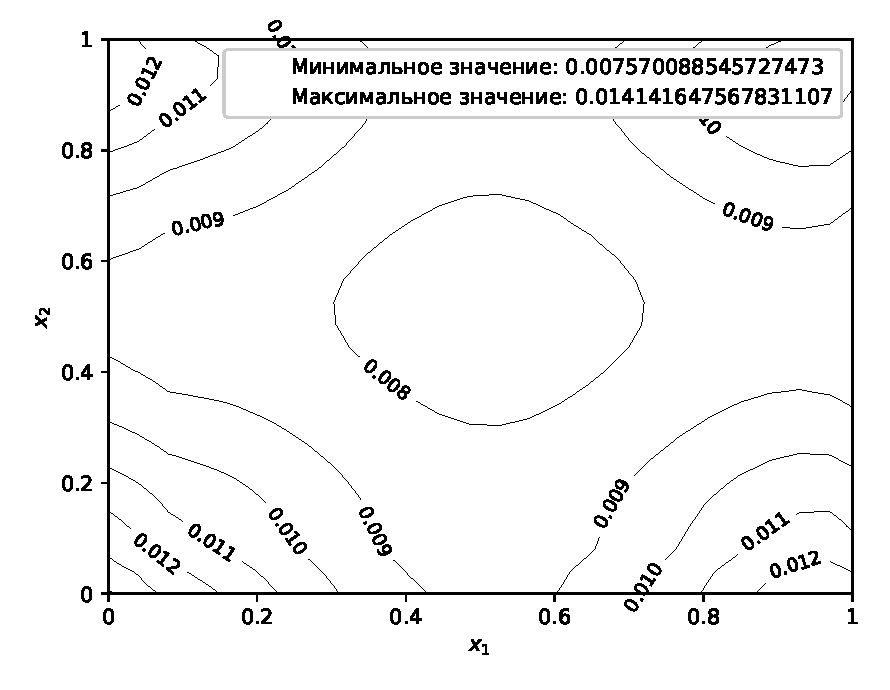
\includegraphics[width=.49\linewidth]{img/exp1/theta_n_diff_iso} }
    \subfloat[Изменение функционала качества по итерациям]
    {\label{fig:quality_1}  \includegraphics[width=.49\linewidth]{img/exp1/quality} }
    \caption{Результаты первого эксперимента}
\end{figure}

\textbf{Пример 2.}
Сравним работу предложенного алгоритма с результатами статьи~\cite{CNSNS19},
где соавтором был один из авторов данной работы.
Задача рассматривается в области $\Omega \times (-L,L)$,
где $\Omega = \{ x = (x_1,x_2) \colon 0 < x_{1,2} < d\}$
и при больших $L$ сводится к двумерной задаче с вычислительной областью $\Omega$.
Выбраны следующие значения параметров задачи:
$d = \mathrm{1(m)}$, $a = 0.92~10^{-4}~\mathrm{(m^2/s)}$, $b= 0.19~\mathrm{(m/s)}$,
$\alpha = 0.0333~\mathrm{(m)}$ и $\kappa_a = 1~\mathrm{(m^{-1})}$.
Параметры соответствуют воздуху при нормальном атмосферном давлении и температуре 400$^\circ$C\@.

Функции $\theta_b$, $q_b$ в краевом условии~\eqref{bc2} заданы следующим образом:
$\theta_b = \widehat{\theta}|_{\Gamma}$, $q_b = \partial_n \widehat{\theta}|_{\Gamma}$, где
$\widehat{\theta} = (x_1-0.5)^2 - 0.5x_2+0.75$.

Приближенное решение задачи с данными Коши, представленное в~\cite{CNSNS19}
получено путем решения эллиптической задачи четвертого
порядка для температуры методом установления по времени.
Использовались $H^2$ конформные конечные элементы Богнера-Фокса-Шмитта и
солвер FeliCs, разработанный в техническом университете Мюнхена.
Решение стабилизировалось через 120 секунд, но вычисления на каждом временном
шаге потребовали довольно значительных затрат~\cite{CNSNS19}.

На рис.~\ref{fig:theta_auto_2} представлено температурное поле, полученное
предложенным в данной статье методом, достаточно точно совпадающее с результатом в~\cite{CNSNS19}.
Величина $\|\partial_n\theta_\lambda-q_b\|_{L^2(\Gamma)}/\|q_b\|_{L^2(\Gamma)}$ равна $~0.000567$.
Значение функционала качества, определяющего норму разности $\|\theta_\lambda -\theta_b\|^2_\Gamma$,
равно $~0.000255$ и стабилизируется после 10 итераций~\ref{fig:quality_2}.

\begin{figure}[H]
    \centering
    \subfloat[Полученное решение $\theta$]
        { \label{fig:theta_auto_2} 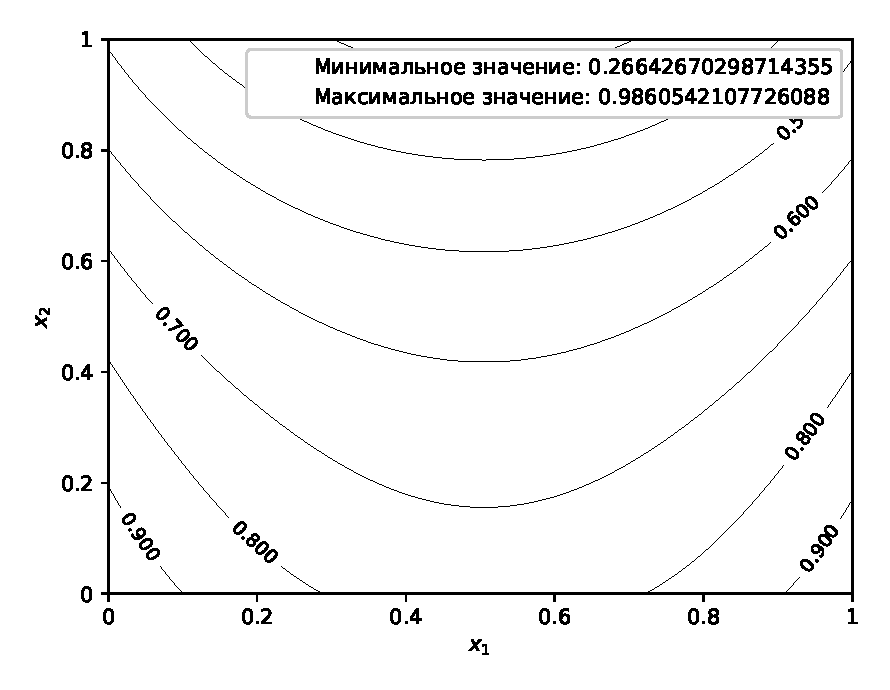
\includegraphics[width=.49\linewidth]{img/exp2/theta_auto} }
    \subfloat[Изменение функционала качества]
    { \label{fig:quality_2} \includegraphics[width=.49\linewidth]{img/exp2/quality} }
    \caption{Результаты второго эксперимента}
\end{figure}

Представленные численные примеры иллюстрируют, что предложенный алгоритм успешно справляется
с нахождением численного решения задачи~\eqref{eq1}-\eqref{bc2}.
%! Suppress = LineBreak
